\documentclass{classrep}
\usepackage[utf8]{inputenc}
\usepackage{color}
\usepackage{graphicx}

\studycycle{Informatyka, studia NIESTACJONARNE, I st.}
\coursesemester{VI}

\coursename{Komputerowe systemy rozpoznawania}
\courseyear{2021/2022}

\courseteacher{dr inż. Marcin Kacprowicz}
\coursegroup{niedziela, 8:00}

\author{
  \studentinfo{Przemysław Lis}{229940} \and
  \studentinfo{Paweł Cichocki}{150848} }

\title{Projekt 1. Klasyfikacja dokumentów tekstowych}

\begin{document}
\maketitle

Opis projektu ma formę artykułu naukowego lub raportu z zadania
badawczego/doświadczalnego/obliczeniowego (wg indywidualnych potrzeb związanych np. z
pracą inżynierską/naukową/zawodową). Kolejne sekcje muszą być numerowane i
zatytułowane. Wzory są numerowane, tablice są numerowane i podpisane nad
tablicą, rysunki sa numerowane i podpisane pod rysunkiem. Podpis rysunku i
tabeli musi być wyczerpujący (nie ogólnikowy), aby czytelnik nie musiał sięgać do tekstu, aby go
zrozumieć.\\
\indent {\bf Wybrane sekcje (rozdziały sprawozdania) są uzupełniane wg wymagań w
opisie Projektu 1. i Harmonogramie Zajęć na WIKAMP KSR jako efekty zadań w~poszczególnych tygodniach}. 

\section{Cel projektu}
Celem projektu jest sparsowanie danych i przeanalizowanie do jakiego kraju odnosi się 
dany artykuł. Do wykonania zadania wykorzystamy algorytm k-NN aby należycie dopasować
kraj. Oczekujemy że nasz program po analizie danych algorytmem będzie w stanie poprawnie
dopasować kraj o którym mowa lub z którego pochodzi artykuł.\\
\noindent


\section{Klasyfikacja nadzorowana metodą $k$-NN}
k-NN jest to algorytm  regresji nieparametrycznej. Założeniem algorytmu jest że podobne problemy mają podobne rozwiązania. Algorytm sprawdza n najbliższych sąsiadów wystąpienia i w zalezności od wyniku klasyfikuje jego położenie. Jeżeli w sąsiedztwie naszego artykułu badawczego będzie najwięcej węzłów danego typu, to wtedy zostanie on odpowiednio dopasowany do danego typu.
Parametrem wejściowym jest plik tekstowy, który następnie będzie zaklasyfikowany do odpowiedniego kraju.\\
\noindent

\subsection{Ekstrakcja cech, wektory cech}
1. Najwięcej wyrazów w pierwszych 5 zdaniach.\\
\begin{displaymath}
\sum_{i = 0}^{5} s_i \textrm{, gdzie s - słowo}\\
\end{displaymath}

2. Stosunek liczby wystąpień słów kluczowych do długości tekstu.\\
\begin{displaymath}
\frac{\sum_{i=0}^{n}s_i}{d}\textrm{, gdzie s - słowo kluczowe, d - długość tekstu}
\end{displaymath}
3. Długość artykułu.\\
\begin{displaymath}
\sum_{i = 0}^{n} l_i \textrm{, gdzie l - litera}\\
\end{displaymath}
4. Średnia dlugość słowa.\\
\begin{displaymath}
\frac{\sum_{i=0}^{n}l_i}{\sum_{j=0}^{n}s_j}\textrm{, gdzie l - litera, s - słowo}
\end{displaymath}
5. Liczba unikalnych słów.\\
\begin{displaymath}
\sum_{i = 0}^{n} s_i \textrm{, gdzie s - słowo unikalne}\\
\end{displaymath}
6. Liczba słów zaczynająca się dużą literą.\\
\begin{displaymath}
\sum_{i=0}^{n}s_i \textrm{,gdzie s - słowo zaczynające się na wielką literę}
\end{displaymath}
7. Liczba słów nie przekraczająca 3 znaków.\\
\begin{displaymath}
\sum_{i=0}^{n}len(s_i)<= 3 \textrm{,gdzie s - słowo}
\end{displaymath}
8. Liczba słów.\\
\begin{displaymath}
\sum_{i = 0}^{n} s_i \textrm{, gdzie s - słowo}\\
\end{displaymath}
9. Liczba słów dłuższych niż 8 znaków.\\
\begin{displaymath}
\sum_{i=0}^{n}len(s_i) > 8 \textrm{,gdzie s - słowo}
\end{displaymath}
10. Litera na którą zaczyna się najwięcej słów z wielkiej litery \\ 
\noindent

\subsection{Miary jakości klasyfikacji} 
{\bf Accuracy} - to miara która określa dokładność klasyfikacji. Jest to stosunek ilości poprawnie zaklasyfikowanych artykułów do wszystkich artykułów. \\
Określona wzorem:
\begin{displaymath}
accuracy = \frac{\textrm{liczba poprawnie zaklasyfikowanych artykułów}}{\textrm{liczba wszystkich artykułów}}
\end{displaymath}

{\bf Precision} - to miara określająca precyzję klasyfikacji elementów do danej klasy. Liczona jest tak jak accuracy, lecz w obrębie pewnej klasy.\\
Określa się wzorem:
\begin{displaymath}
precision = \frac{\textrm{liczba poprawnie zaklasyfikowanych artykułów do klasy X}}{\textrm{liczba wszystkich artykułów zaklasyfikowanych do klasy X}}
\end{displaymath}

{\bf Recall} - jest to miara oznaczająca odsetek poprawnie zaklasyfikowanych artykułów do danej klasy.\\
Określa się wzorem:
\begin{displaymath}
recall = \frac{\textrm{liczba poprawnie zaklasyfikowanych artykułów do klasy X}}{\textrm{liczba wszystkich artykułów klasy X}}
\end{displaymath}

{\bf F1} - jest to miara uśredniająca wynik. Liczona jest poprzez średnią harmoniczną precision oraz recall.\\
Określa się wzorem:
\begin{displaymath}
F1 = 2 \cdot  \frac{precision \cdot recall}{precision + recall}
\end{displaymath}


\section{Klasyfikacja z użyciem metryk i miar podobieństwa tekstów}
Wzory, znaczenia i opisy symboli zastosowanych metryk z
przykładami. Wzory, opisy i znaczenia miar
podobieństwa tekstów zastosowanych w obliczaniu metryk dla wektorów cech z
przykładami dla każdej miary \cite{niewiadomski08}.  Oznaczenia jednolite w obrębie całego sprawozdania.  Wstępne wyniki miary Accuracy dla próbnych klasyfikacji na ograniczonym zbiorze tekstów (podać parametry i kryteria
wyboru wg punktów 3.-8. z opisu Projektu 1.). {\bf Podaj metryki i miary
podobieństwa nie z literatury (te wystarczy zacytować linkiem), ale konkretne ich
postaci stosowane w zadaniu. Jakie zakresy wartości przyjmują te miary i
metryki, co oznaczają ich wartości? Podaj przykładowe wartości dla przykładowych wektorów cech}. \\ 
\noindent {\bf Sekcja uzupełniona jako efekt zadania Tydzień 04 wg Harmonogramu Zajęć
na WIKAMP KSR.}

\section{Budowa aplikacji}
\subsection{Diagramy UML}
Program będzie posiadł klasę Main króta będzie zarządzać całym programem. Będą do niej dołączone klasy takie jak Algorithms, LoadData czy Characteristic. Do załadowania plików posłuży nam klasa LoadData, która będzie ładować artykuły do klasy Article za pomocą paternu z klasy SGAFileNormalizer.
klasyfikatora.\\
\begin{figure}[!htbp]
	\centering
     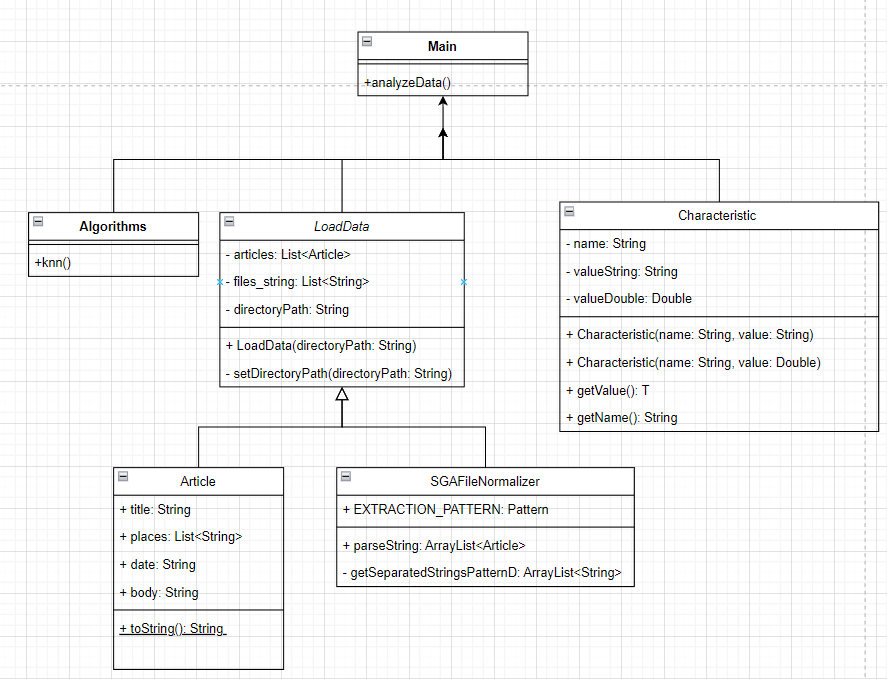
\includegraphics[width=\textwidth]{img/uml.png}
	\caption{Diagram UML całego projektu}
\end{figure}



\subsection{Prezentacja wyników, interfejs użytkownika} 
Krótki ilustrowany opis jak użytkownik może korzystać z aplikacji, w~szczególności wprowadzać parametry klasyfikacji i odczytywać wyniki. Wersja JRE i inne wymogi
niezbędne do uruchomienia aplikacji przez użytkownika na własnym komputerze. \\
\noindent {\bf Sekcja uzupełniona jako efekt zadania Tydzień 04 wg Harmonogramu Zajęć
na WIKAMP KSR.}

\section{Wyniki klasyfikacji dla różnych parametrów wejściowych}
Wyniki kolejnych eksperymentów wg punktów 2.-8. opisu projektu 1.  Wykresy i tabele
obowiązkowe, dokładnie opisane w ,,captions'' (tytułach), konieczny opis osi i
jednostek wykresów oraz kolumn i wierszy tabel.\\ 

{**Ewentualne wyniki realizacji punktu 9. opisu Projektu 1., czyli,,na ocenę 5.0'' i ich porównanie do wyników z
części obowiązkowej**.}\\

\noindent {\bf Sekcja uzupełniona jako efekt zadania Tydzień 05 wg Harmonogramu Zajęć
na WIKAMP KSR.}


\section{Dyskusja, wnioski}
Dokładne interpretacje uzyskanych wyników w zależności od parametrów klasyfikacji
opisanych w punktach 3.-8 opisu Projektu 1. 
Szczególnie istotne są wnioski o charakterze uniwersalnym, istotne dla podobnych zadań. 
Omówić i wyjaśnić napotkane problemy (jeśli były). Każdy wniosek/problem powinien mieć poparcie
w przeprowadzonych eksperymentach (odwołania do konkretnych wyników: wykresów,
tabel). \\
\underline{Dla końcowej oceny jest to najważniejsza sekcja} sprawozdania, gdyż prezentuje poziom
zrozumienia rozwiązywanego problemu.\\

** Możliwości kontynuacji prac w obszarze systemów rozpoznawania, zwłaszcza w kontekście pracy inżynierskiej,
magisterskiej, naukowej, itp. **\\

\noindent {\bf Sekcja uzupełniona jako efekt zadania Tydzień 06 wg Harmonogramu Zajęć
na WIKAMP KSR.}


\section{Braki w realizacji projektu 1.}
Wymienić wg opisu Projektu 1. wszystkie niezrealizowane obowiązkowe elementy projektu, ewentualnie
podać merytoryczne (ale nie czasowe) przyczyny tych braków. 


\begin{thebibliography}{0}
\bibitem{tadeusiewicz90} R. Tadeusiewicz: Rozpoznawanie obrazów, PWN, Warszawa, 1991.  
\bibitem{niewiadomski08} A. Niewiadomski, Methods for the Linguistic Summarization of Data: Applications of Fuzzy Sets and Their Extensions, Akademicka Oficyna Wydawnicza EXIT, Warszawa, 2008.
\end{thebibliography}

Literatura zawiera wyłącznie źródła recenzowane i/lub o potwierdzonej wiarygodności,
możliwe do weryfikacji i cytowane w sprawozdaniu. 
\end{document}
